\documentclass[twocolumn]{article}

\usepackage{enumerate}
\usepackage{graphicx}
\usepackage[colorlinks=true,linkcolor=blue]{hyperref}
\usepackage[table,xcdraw]{xcolor}
\usepackage[english,spanish]{babel} 
\usepackage{helvet}

\renewcommand{\familydefault}{\sfdefault}

\newenvironment{poliabstract}[1]
   {\renewcommand{\abstractname}{#1}\begin{abstract}}
   {\end{abstract}}

\begin{document}

\title{Datos no estructurados}
\author{Herrera Amezquita,
Derian  \\Paredes Catacora, Randi \\Mejia Rodriguez, Julio\\Abraham Lipa Calabilla}


\date{05 de Enero del 2021}

\maketitle

\selectlanguage{spanish}
\begin{poliabstract}{Resumen} 
  En el desarrollo del articulo de investigacion expondremos sobre las formas de extracción de datos no estructurados.
  
\end{poliabstract}

\selectlanguage{english}
\begin{poliabstract}{Abstract} 
  In the development of the research article we will expose on the forms of extraction of unstructured data.
\end{poliabstract}

\section{Introducción}
Una gran mayoría es decir 80\% de datos en el mundo actual no está estructurado y este número continúa 
creciendo rápidamente. Para ilustrar más sobre esta estadística, las bases de datos empresariales estructuradas
 pueden constar de hasta decenas de terabytes de datos (incluidas copias de seguridad y registros duplicados).
  Pero cuando hablamos de conjuntos de datos no estructurados, como los generados a partir de dispositivos IoT, 
  el tamaño puede estar en exabytes (millones de terabytes). Este gran volumen y complejidad son factores que 
  hacen que la gestión de datos no estructurados (UDM) sea una tarea difícil.

\section{Desarrollo}
\subsection{¿Qué son los datos no estructurados?}
Los datos no estructurados pueden definirse como datos, en cualquier forma, que no tengan un modelo o formato 
predefinido. Este tipo de datos se genera a partir de varias fuentes, incluidos audio, video, imágenes y texto.
La mayoría de las organizaciones cuentan con estrategias sólidas para administrar y analizar sus datos estructurados,
 pero el valor real radica en administrar esta nueva ola de contenido no estructurado. En esta publicación de blog, 
 presentamos los fundamentos de las soluciones de administración de datos no estructurados para equipos de TI y 
 propietarios de negocios.[1]

\subsection{Gestión de datos no estructurados oportunidades disponibles}
Al analizar los datos no estructurados, las empresas pueden ver información en nuevas dimensiones que mejoran 
enormemente la toma de decisiones. Aquí hay dos áreas clave en las que la gestión de datos no estructurados puede 
resultar beneficiosa:
\textbf{* Inteligencia de negocios}\\
Un buen enfoque de la inteligencia empresarial es utilizar datos de fuentes internas y
 externas para el análisis. Es fácil acceder a datos estructurados desde una base de 
 datos interna, pero usar información atrapada en API de terceros y conjuntos de datos 
 de código abierto disponibles en la web es un desafío. Esto se debe a que estos datos 
 deben procesarse antes de ingresar a un sistema de BI. Sin embargo, el uso de datos no
  estructurados puede ayudarlo a evaluar la información desde nuevos ángulos. Por ejemplo, 
  puede identificar los cuellos de botella en el recorrido del comprador del cliente de su 
  tienda en línea mediante el estudio de las interacciones del cliente con una herramienta 
  como Hotjar. Puede utilizar su información para mejorar el diseño general de su sitio web 
  y hacer que las llamadas a la acción sean más efectivas, lo que finalmente tendrá un 
  impacto positivo en la tasa de conversión.\\

  \textbf{* Desarrollo de productos}\\
  Toda organización quiere aprender cómo pueden mejorar su 
  proceso de desarrollo de productos. Capturar y analizar
  datos no estructurados puede ayudar con esto. Por ejemplo,
   si sabía de qué hablaban sus clientes en las redes sociales,
  puede obtener más información sobre sus intereses y patrones
   de comportamiento. El equipo de desarrollo de productos puede
  utilizar toda esta información para lanzar nuevos productos
 y servicios que tengan una gran demanda, lo que eventualmente
   generará mayores ventas.
   
\subsection{Gestión de datos no estructurados: requisitos clave}

\textbf{*Almacenar todo}\\El primer requisito clave para administrar datos no estructurados 
es comenzar a almacenar todas datos que genera, sin importar de qué forma sean o de 
dónde provengan. Con el costo del almacenamiento de datos cada vez más barato, 
la retención de datos a largo plazo puede costarle unos pocos dólares por terabyte 
anualmente en soluciones de almacenamiento basadas en la nube.\\
\textbf{*Separar datos del almacenamiento}\\
 Ahora que está almacenando toda esta información, 
el siguiente paso es usar estos datos para obtener información. Uso de herramientas 
locales, como ReportMiner, puedo ayudarte extraerlos datos no estructurados de varias 
fuentes y integrar con sus datos estructurados para que tenga toda la información disponible 
para sus herramientas de análisis de datos.\\


\section{¿Qué es Automatic Speech Recognition?}

El \textbf{Reconocimiento automático del habla} es la capacidad que permite a un programa procesar el habla humana en un formato escrito. Si bien comúnmente se confunde con el reconocimiento de voz, el reconocimiento de voz se enfoca en la traducción del habla de un formato verbal a uno de texto, mientras que el reconocimiento de voz solo busca identificar la voz de un usuario individual. [5]

\subsection{Historia}

Entre los hechos históricos que involucran el término Reconocimiento de voz podemos mencionar: [6]

\begin{enumerate}
  \item El primer intento registrado de tecnología de reconocimiento de voz se remonta al año 1000 d.C. a través del desarrollo de un instrumento que supuestamente podría responder "sí" o "no" a preguntas directas. No contaba con un procesamiento de lo que se decía, solo que el lenguaje natural desencadenaba una acción.
  \item Los laboratorios Bell trabajaron para desarrollar "Audrey", un sistema capaz de reconocer los números del 1 al 9 hablados por una sola voz.
  \item IBM desarrolló un dispositivo que podía reconocer y diferenciar entre 16 palabras habladas.
  \item El 4 de octubre de 2011 se anunció que Siri se incluiría con el iPhone 4S.
  \item El 2 de abril de 2014, Cortana se demostró por primera vez en la Conferencia de desarrolladores de Microsoft BUILD.
  \item En noviembre de 2014, Amazon anunció Alexa junto a Echo.
\end{enumerate}

\subsection{Características}

Hay muchas aplicaciones y dispositivos de reconocimiento de voz disponibles, pero las soluciones más avanzadas utilizan inteligencia artificial y aprendizaje automático que permiten una mejor detección de:

\begin{itemize}
  \item gramática
  \item sintaxis
  \item estructura
  \item composición
\end{itemize}

De las señales de audio y voz para comprender y procesar el habla humana. Idealmente, aprenden sobre la marcha, evolucionando las respuestas con cada interacción.

\begin{description}
  \item Ponderación del idioma: \\
        Precisión de la ponderación de palabras específicas, no se limita al vocabulario básico.
  \item Etiquetado de oradores: \\
        Identificación y etiquetado de diferentes oradores en un grupo.
  \item Formación en acústica: \\
        Adaptación al entorno acústico.
  \item Filtrado de blasfemias: \\
        Filtro de ciertas palabras.
\end{description}

En la actualidad, el software de reconocimiento de voz de Google se está acercando a la precisión del nivel humano, llegando al 95\% de precisión gracias a algoritmos de Machine Learning. [7]

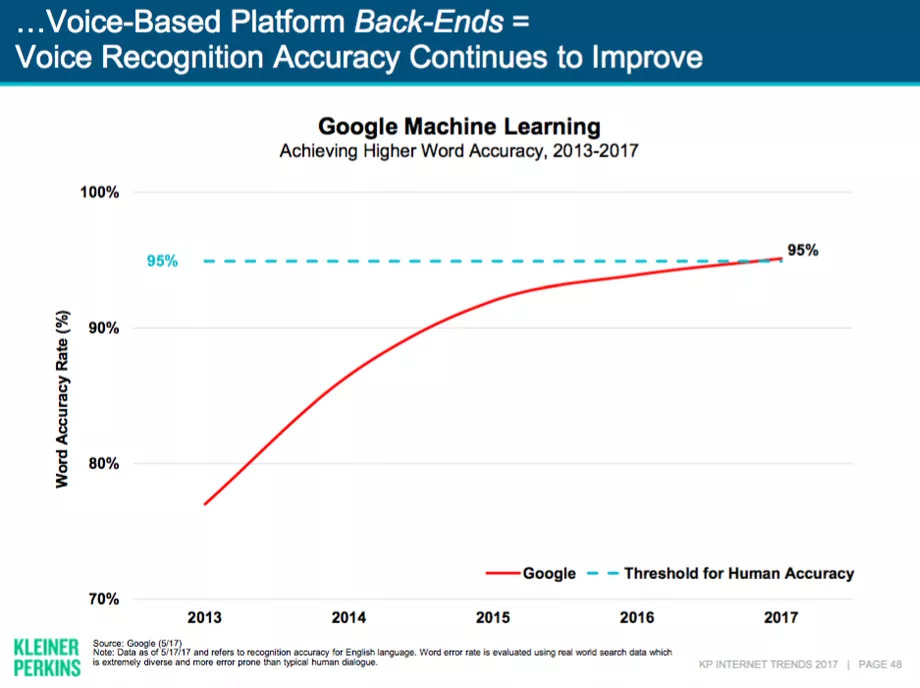
\includegraphics[width=1.02\linewidth]{img/aagyw-j4rrq.jpg}

\subsection{Natural Language Processing (NLP)}

Es el área de la inteligencia artificial que se centra en la interacción entre humanos y máquinas a través del lenguaje a través del habla y el texto. Muchos dispositivos móviles incorporan el reconocimiento de voz en sus sistemas para realizar búsquedas por voz.

\subsection{Algoritmos}

\subsubsection{Hidden Markov Models}

Se basan en el modelo de cadena de Markov, que estipula que la probabilidad de un estado dado depende del estado actual, no de sus estados anteriores. Si bien un modelo de cadena de Markov es útil para eventos observables, como entradas de texto, los modelos de Markov ocultos nos permiten incorporar eventos ocultos, como etiquetas de parte del discurso, en un modelo probabilístico. [5]

\subsubsection{Neural Networks}

Principalmente aprovechadas para algoritmos de Deep Learning, las redes neuronales procesan los datos de entrenamiento imitando la interconectividad del cerebro humano a través de capas de nodos. Cada nodo está formado por entradas, pesos, un sesgo (o umbral) y una salida. Si ese valor de salida excede un umbral dado, "dispara" o activa el nodo, pasando datos a la siguiente capa en la red. Si bien las redes neuronales tienden a ser más precisas y pueden aceptar más datos, esto tiene un costo de eficiencia en el rendimiento, ya que tienden a ser más lentas de entrenar en comparación con los modelos de lenguaje tradicionales. [5]

\subsubsection{Speaker Diarization (SD)}

Los algoritmos de registro del hablante identifican y segmentan el habla según la identidad del hablante. Esto ayuda a los programas a distinguir mejor a las personas en una conversación. [5]

\section{¿Computer Vision que es?}
es una disciplina científica que incluye métodos para adquirir, procesar,
 analizar y comprender las imágenes del mundo real con el fin de producir información
  numérica o simbólica para que puedan ser tratados por un ordenador. Tal y como los 
  humanos usamos nuestros ojos y cerebros para comprender el mundo que nos rodea, la 
  visión artificial trata de producir el mismo efecto para que los ordenadores puedan 
  percibir y comprender una imagen o secuencia de imágenes y actuar según convenga en 
  una determinada situación. Esta comprensión se consigue gracias a distintos campos 
  como la geometría, la estadística, la física y otras disciplinas.
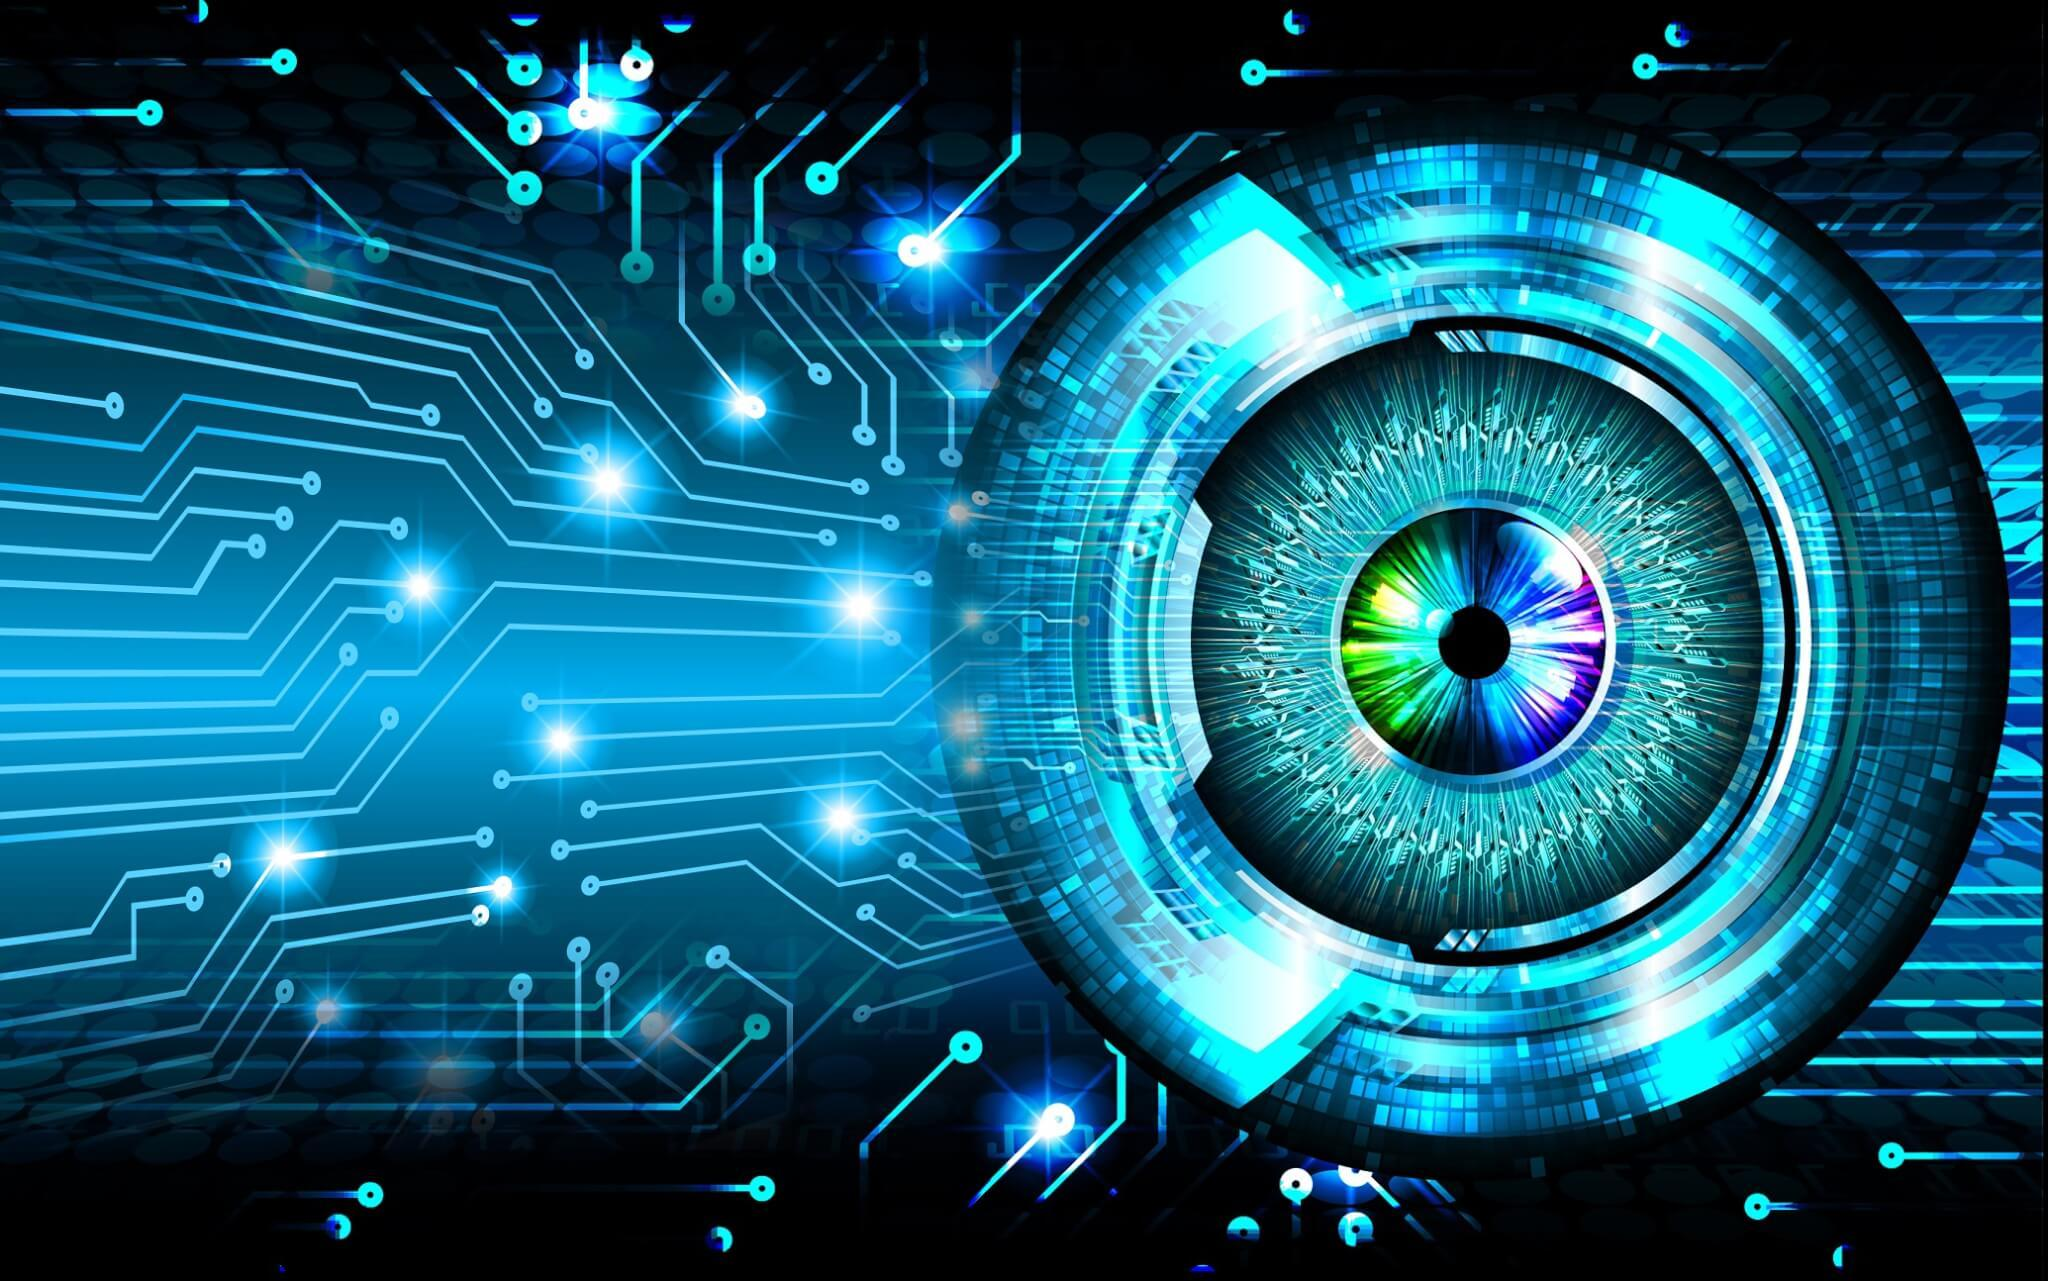
\includegraphics[width=1.02\linewidth]{img/vs.jpg}
  
  \subsection{Aprendizaje automatico}
Las técnicas de aprendizaje automático tienen como objetivo conseguir diferenciar 
automáticamente patrones usando algoritmos matemáticos. Estas técnicas son comúnmente 
usadas para clasificar imágenes, para tomar decisiones dentro del mundo empresarial 
(por ejemplo, para decidir qué clientes de un banco pueden recibir un préstamo o cuánto 
ha de pagar cada cliente por un seguro dependiendo de sus antecedentes), así como dentro 
de muchos otros ámbitos de la ciencia y la tecnología. Principalmente se pueden distinguir 
dos tipos de técnicas: supervisadas y no supervisadas.
En el aprendizaje supervisado se entrena al ordenador proporcionando patrones previamente 
etiquetados, de forma que algoritmo usado debe encontrar las fronteras que separan los posibles 
diferentes tipos de patrones. Adaboost y algunas redes neuronales forman parte de este grupo.
En el aprendizaje no supervisado se entrena al ordenador con patrones que no han sido 
previamente clasificados y es el propio ordenador el que debe agrupar los distintos patrones 
en diferentes clases. K-means y algunas redes neuronales forman parte de este grupo.
Ambas técnicas son muy utilizadas en la visión artificial, sobre todo en clasificación y 
segmentación de imágenes.[3]
\subsection{Detección de objetos}
La detección de objetos es la parte de la visión artificial que estudia cómo detectar la presencia de objetos en una imagen sobre la base de su apariencia visual, bien sea atendiendo al tipo de objeto (una persona, un coche) o a la instancia del objeto.
Generalmente se pueden distinguir dos partes en el proceso de detección: la extracción de características del contenido de una imagen y la búsqueda de objetos basada en dichas características.
La extracción de características consiste en la obtención de modelos matemáticos compactos que "resuman" el contenido de la imagen con el fin de simplificar el proceso de aprendizaje de los objetos a reconocer. Dichas características son comúnmente llamadas descriptores.
Existen diversos tipos de descriptores, que tendrán mejor o peor rendimiento en función al tipo de objeto a reconocer y a las condiciones del proceso de reconocimiento (la luz controlada o no, distancia al objeto a reconocer conocida o no). Se pueden usar desde básicos histogramas de color o intensidad de luz, descriptores LBP (Local Binary Pattern, usado sobre todo para texturas) o más avanzados como el HOG (Histogram of Oriented Gradientes) o SIFT.[4]
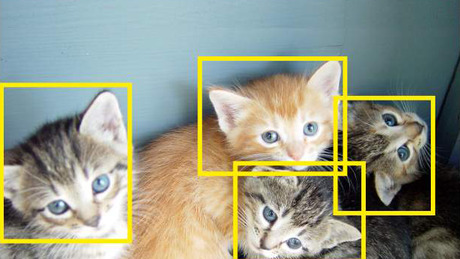
\includegraphics[width=1.02\linewidth]{img/deteccion.jpg}

\subsection{Análisis de video}
El análisis de vídeo es fundamental en el sector de vídeo vigilancia y seguridad. En un sistema de CCTV(circuito cerrado de televisión) tradicional es habitual visualizar el contenido de hasta 16 cámaras simultáneamente. Esta tarea resulta complicada para un vigilante de seguridad pues hay estudios que aseguran que después de 22 minutos de supervisión este pierde hasta el 95 por ciento de la actividad de la escena. Con el análisis de vídeo se alerta al vigilante cuando hay movimiento o señala en qué cámara hay mayor probabilidad de actividad sospechosa o peligrosa.
Una de las capacidades básicas del análisis de vídeo es la detección de movimiento: tecnología que identifica y alerta cuando ocurre el movimiento. Sofisticadas adaptaciones de la detección de movimiento incluyen sensores que detectan el movimiento en direcciones no autorizadas.
\\
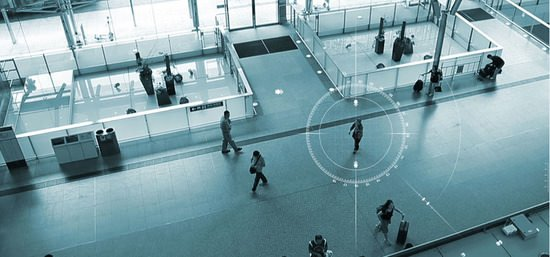
\includegraphics[width=1.02\linewidth]{img/video.jpg}
\section{Bibliografía}

\begin{thebibliography}{X}
  
  
  \bibitem{Baz} \textsc{netapp} ,
  \textit{}(2019)¿Qué son los datos no estructurados?\url{https://www.netapp.com/es/data-storage/unstructured-data/what-is-unstructured-data/}
  
  \bibitem{Baz} \textsc{Astera.com} ,
  \textit{}(2019),Machine Learning in Computer Vision\url{https://www.cs.princeton.edu/courses/archive/spring07/cos424/lectures/li-guest-lecture.pdf}


  \bibitem{Baz} \textsc{princeton.edu} ,
  \textit{}(2018)¿Qué son los datos no estructurados?\url{https://www.netapp.com/es/data-storage/unstructured-data/what-is-unstructured-data/}
  
  \bibitem{Baz} \textsc{Coursera} ,
  \textit{}(2018)Detección de objetos\url{https://www.coursera.org/learn/deteccion-objetos}

  [5] https://www.ibm.com/cloud/learn/speech-recognition

  [6] https://www.globalme.net/blog/the-present-future-of-speech-recognition/

  [7] https://www.vox.com/2017/5/31/15720118/google-understand-language-speech-equivalent-humans-code-conference-mary-meeker



\end{thebibliography}


\end{document}